\chapter[SCP-001 一致意见]{
	SCP-001 Wrong - The Consensus \\
	SCP-001 一致意见
	\footnote{编者\QIS:这个脚注用于去除一个我还没搞明白的\TeX 排版问题,只要标题的最后一个字不是汉字就行,为了美观就加了个脚注\label{foot:fix}}
}

\label{chap:SCP-001.the.consensus}

\definecolor{ftwoftwoctwo}{HTML}{F2F2C2}

\begin{scpbox}[colback=ftwoftwoctwo, center upper]

\bb{基金会记录与信息安保管理部通知}

一年二度安保更新:项目编号随机化已启动。直至安保更新完成,所有文件将锁定。要进行紧急更新,请访问紧急数据归档系统(EDAS)。

— Maria Jones,RAISA主管

\end{scpbox}

\hr

\begin{scpboxcmd}

> 1908个项目存留。项目编号“SCP-001”锁定。 \\
> 识别到1个带有搜索字段“SCP-001”的文件。

> 文件~'SCP-001'被选中。 \\
> 开始自动项目编号随机化。 \\
> 扫描带有搜索字段“SCP-001”的文件…

\end{scpboxcmd}

\hr

\begin{figure}[H]
	\centering
	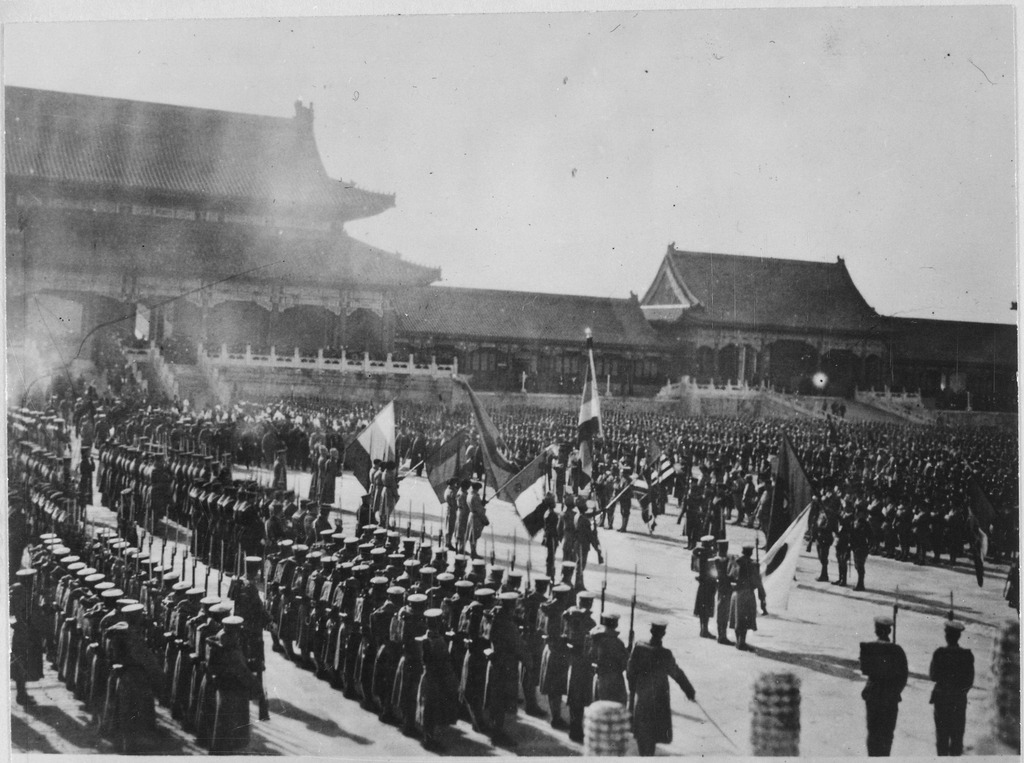
\includegraphics{images/SCP.001.the.consensus.jpg}
	\caption*{北京紫禁城,\red{SCP-001}的定义及紫禁城公约的通过在此完成。}
\end{figure}

\bb{项目编号:}\red{SCP-001}

\bb{项目等级:}Euclid

\bb{权限分级:}5级

\bb{特殊收容措施:}\red{SCP-001}当前无法被便利控制或收容,未知其是否会在未来发生。因此已采用应对方案。该方案由紫禁城公约的以下章节组成:

\begin{enumerate}
\item 依照紫禁城公约章节I,预防并最小化可能造成\red{SCP-001}或类似事件的情形。
\item 在紫禁城公约章节I实施后,依照紫禁城公约章节II及III安排组织过渡及联合。
\end{enumerate}

上述紫禁城公约章节不得变动,除非得到O5议会全体一致通过。

描述:\red{SCP-001}是一已经发生的CK级重构情形,造成过往某一迭代的现实变化,生成了当前的现实。从第一人称观察记录来看,\red{SCP-001}发生于前现实的公元1900年6月1日。\red{SCP-001}致使所有关于超自然大战\ii{i}(前一现实中称其为第五次超自然大战)的因果、事件、记载和记忆被删除并替代为各种异常或非异常的平行记录。

基金会关于超自然大战\ii{i}的文件采集自十三名非异常人类的传闻记录,这些人员因被称作“部分性\red{SCP-001}免疫”的现象而保有对前一现实的记忆。部分性\red{SCP-001}免疫的原理未知,依照O5议会指令不会对其进行评定。依照O5议会指令,对其他具有部分性\red{SCP-001}免疫人员的辨识工作被无限期暂停。

下面是在超自然大战\ii{i}中的事件及其在当前现实中可能的对应类似事件;参见文件OWi获取完整列表。

\tred{+ 查看列表}

\tred{- 隐藏列表}

\begin{longtable}{m{0.2\linewidth}m{0.3\linewidth}m{0.35\linewidth}}
\hline
超自然大战\ii{i}事件 & 描述 & 当前现实对应 \\
\hline
\endhead
\hline
\multicolumn{3}{r}{\small{接下页}}
\endfoot
\hline
\endlastfoot
“第五次超自然大战”的称谓 & 发生于公元19世纪的全球性战争,由发生于欧洲(拿破仑战争)、东亚(狄瓦族征服战)及美洲(美国内战)的三起独立冲突组成。战争中公然使用异常物体,造成了一次IK级全球文明崩溃情景。 & 与“拳乱”同时发生于中国北部的冲突事件,起义组织义和团据称在此事件中使用了某种未命名异常。\par 虽然对异常的使用非常微小,O5议会仍在知晓异常现象的诸组织中倡议将“第五次超自然大战”作为对此事件的正式称呼,全球超自然联盟在基金会-GOC的1953年峰会中正式承认了这一主张。\\
拿破仑一世加冕 & 拿破仑皇帝在加冕后宣布新诺斯替教为法国国教,欧罗巴为国家守护神。& 教皇庇护七世将拿破仑加冕为“法兰西皇帝”拿破仑统治期间从未有发现过新诺斯替主义和欧罗巴女神崇拜的表现。 \hyperref[chap:SCP-2515]{SCP-2515}是对此的唯一证据。\\
狄瓦族东亚征服战	& 东亚大部分地区被名为\overtextnote{\hyperref[chap:SCP-140]{狄瓦族}(\footnotesize{Daevites})}的类人文明入侵。征服从中国黑龙江省及吉林省开始。& 没有对应事件。\hyperref[chap:SCP-140]{SCP-140}中的记录显示狄瓦文明被蒙古人消灭于公元13世纪。然而,确实曾在中国黑龙江省及吉林省发现过狄瓦文明器物。\\
南北战争 & 美利坚合众国及美国南部邦联间的内战。名为“工厂”的团体向双方都提供了异常军备支援。在南部邦联政府转移后,战争逐步扩展到墨西哥、中南美。& 未发现工厂参与南北战争。战争规模始终局限于美国大陆地区。\\
图基教平定运动 & 第零反邪教军团针对骚扰\hyperref[chap:SCP-2833]{Vātula}(被视作与英国东印度公司对抗狄瓦族对印度入侵的共同战力)的犯罪集团图基教的镇压活动。& 由《1836-48年图基教及土匪镇压法案》委任的镇压活动,确认有新欲肉教参与。\\
梵蒂冈神秘及预言圣裁庭 & 知晓异常现象的组织,隶属于梵蒂冈圣座。在拿破仑进攻意大利半岛时,其成员逃难到南美、非洲自由邦及中东。& 圣物部(梵蒂冈圣裁庭下属部门)叛逃到意大利统一政府,组建了基金会前身组织之一“皇家基督教圣物办公室”。\hyperref[chap:SCP-1732]{梵蒂冈圣裁庭在公元1964年与基金会合并}。\\
“墨西哥帝国”的建立 & 自称Cem Anáhuac,是阿兹特克帝国的后继者。\hyperref[chap:2155]{其对象及由其产生的媒体具有模因能力},被用于政府周边邦国,如德克萨斯、危地马拉、萨尔瓦多和洪都拉斯。& 墨西哥第二帝国在法国干涉下建立,由皇帝马西米兰一世统治。据传他在被处决前曾与一个SCP-2155-1个体安排了联姻。\\
东田纳西会议 & 由东田纳西的合众国支持者组成,在田纳西州参与南北战争后脱离该州。由此形成的\hyperref[chap:SCP-1328]{富兰克林州}被承认加入美利坚合众国,也是合众国一方中唯一一个自南部邦联脱离的州。& 东田纳西会议在南方军占领东田纳西后告终。西弗吉尼亚自弗吉尼亚州脱离,并在南北战争后作为一个州保留。\\
太平天国运动 & 在狄瓦占领下的中国南部发生,由一名为洪仁坤的奴隶策划发起,他自称得到了名为\hyperref[doc:2481]{“龙母”}的神明启示。在起义首都太岁京(被太平军占领前为南京)被狄瓦族攻陷后遭到镇压,全城居民被屠杀。& \hyperref[chap:SCP-089]{SCP-089}告知的一起S级事件,由女王陛下超常控制收容基金会及黑庄园的联合探险队处置解决。洪仁坤在此利用了对基督教的自我改造,并给自己改名为洪秀全。\par 未发现欲肉教或基督教相关异常活动涉及此事。南京在被太平军占领后改名为天京。\\
土默特部大屠杀 & 一名狄瓦族奴隶在狄瓦占领下的蒙古地区系统性屠杀了150000名蒙古人。报告称\hyperref[chap:SCP-076]{此奴隶}手持两把带刃武器并具有某种再生能力。起义者的尸体被狄瓦军队以未知目的回收。& 一起“金丹道之乱”类似地造成了150000名蒙古人被屠杀,但此事是由中国秘密结社金丹道造成。金丹道在前一现实的存在因资源有限而无法确认。
\end{longtable}

\red{SCP-001}的起因和源头未知,也无法确认。未知\red{SCP-001}或类似事件在此之前是否还曾发生,也未知其是否会在未来发生。此外,未知\red{SCP-001}是否是CK级重构情景的典型或非典型表现。若\red{SCP-001}或类似事件已经发生或是将要发生,推测大部分(甚至全部)人类和/或智能实体将对此事件及其发生前的事件不会保留记忆。无法确认部分性\red{SCP-001}免疫是否能在未来的\red{SCP-001}或其类似事件中有效。

\red{SCP-001}的定义由O5议会以投票5-4-4完成,紫禁城公约于公元1901年9月7日签订。

\bb{附录1:}紫禁城公约摘录

\bb{章节I:基金会}

\begin{whiteboxbb}

下列组织将自各自资助方中解散并脱离关系,其人员及资源将进行合并:

\begin{itemize}
\item 女王陛下超常安保收容基金会
\item \ii{黑}庄园
\item 沙皇先知会
\item 德意志帝国秘传战团
\item 美国安保收容倡议
\item 帝国侵犯事件委员会
\item 皇家基督教圣物办公室
\item 荷兰东印度公司特别调查董事会
\item 内阿非利加探索队会社
\item Borja y Aragón军备骑士团
\item 阴阳局
\item 中华异学会
\item 第零反邪教军团
\end{itemize}

它们将被取而代之联合为一个统一组织。

该统一组织的使命是控制并收容各种异常事物,以保护人类免受此类事物威胁。

同意将该统一组织的称谓定为“基金会”;其他替换称谓(如“学会”、“组织”、“机构”、“前哨”)曾被提议但否决。上述十三个基金会构成组织自此后称作“基金会前身组织”。

\end{whiteboxbb}

\bb{章节II:O5议会}

\begin{whiteboxbb}

基金会的临时执行管理部门将是来自各前身组织的十三名人员组成的执行议会。

上述十三名执行议会成员将依照下列标准选择:

\begin{itemize}

\item 在各基金会前身组织居领导职位
\item 保有关于第一次超自然大战\ii{i}的记忆

\end{itemize}

未来的执行议会成员不再要求满足上述两个要求。

同意将执行议会的称谓定为“O5议会”;其他替换称谓(如“监督者委员会”、“5级议会”、“O5指挥部”)曾被提议但否决。

O5议会的功能将为促进各前身组织间的初步过渡。

每名O5议会成员将以罗马数字编号,从一排列到十三。

今后其他并入基金会的组织机构不得在O5议会存有代表。

\end{whiteboxbb}

\bb{章节III:关注组织}

\begin{whiteboxbb}

知晓异常现象存在而不受基金会管控的各组织机构被编为 \overtextnote{“关注组织”(Groups of Interest)}。

基金会对各关注组织的默认对策是促成其人员和资源的解散、终止和/或将其吸收。

\end{whiteboxbb}

\bb{附录O5-(1-13):}继任笔记re:\red{SCP-001}。 文件根据登录的O5账号显示。

\definecolor{dafadnine}{HTML}{DAFAD9}

\begin{scpboxc}[colback=dafadnine]

验证登录权限。识别到管理员优越权(代号嚎叫黑月)。\\
展示所有文件。

\end{scpboxc}

% \begin{whiteboxbb}

\begin{scpbox}

欢迎您O5-1

致我的继任者,

作为\red{SCP-001}的主要编辑者,我已写下了你所需知晓的一切。在\red{SCP-001}后,只有我们十三个知道它,我们各自代表各自的前身组织。当然,我们命定要指挥和联合为基金会。

你可以从我们的投票看出,我们在北京争论时有关于\red{SCP-001}的另外两种版本。它们最终被投票否决,但二和十二仍在基金会历史上留下了自己的记号。遗憾的是十二有限的英语水平让它选中了相对通俗化的分级名词,与二和我刚好相对。无论如何,我们召开首次O5会面的倡议将在已写下的所有SCP文件中被记忆、发扬。

至于基金会之使命,我希望你和你的同事能继续我们的工作。

\end{scpbox}

\begin{scpbox}

欢迎您O5-2

致我的继任者,

桑塔亚纳曾说,“忘记过去的人必将重蹈覆辙”。现在,整个世界都忘记了过去。但它会重蹈覆辙吗?它会的。

在第二次世界大战期间,不是又有一个威权独裁者恐吓欧洲,中国人再一次被屠杀了吗?当然,细节些许不同,美国也在战争中保持了完整。也许内战在你的一生曾再次发生,或者很快就要发生。又或者缩减为一次小冲突。 工厂仍然留存,但它只是幻影。

异常的产物自身也会是异常。\red{SCP-001}和它的世界不是例外。一点一点,世界在毁灭、重蹈覆辙。每有一个SCP不(或者只是最低程度地)在我们的控制下,这个进程都要继续。在那之前,系统里都会有混乱存在。曾经,我提议指引世界回到原来的状态,但其他人不愿赞成专横暴行。最终,我认了。 没必要为我的观点斗争。没什么能改变这个过程。

除了等待,不必采取任何行动。或者简言之,“Keter”。

\end{scpbox}

\begin{scpbox}

欢迎您O5-3

致我的继任者,

异常与正常—都取决于合意。今日的异常可能是昨日之正常,反之亦然。九未能发觉的丑闻就是一例;出逃狂在合意认为它不再成立后便不再是异常。

将合意适用在\red{SCP-001}。对其余的世界,超自然大战从未存在。它们只对那些知道异常的人存在。对知道异常的人,超自然大战\ii{i}并不存在。只有十三人幻想它存在,那可能就是\red{SCP-001}。

然而,议会建立了我们自己的合意,我的观点在它宣告之时也随之转变。我们多数决定应该对所有异常事务建立管控秩序,而不是觉得我们自己才是问题。这只是第一批达成的合意之一,我们能左右世界将什么视作正常,什么不是。也许是他们造就了你所成长的这个世界。

所以,请记得这些。合意有其价值,要正常就要被合意所接纳。

\end{scpbox}

\begin{scpbox}

欢迎您O5-4

致我的继任者,

只有少数人在两个第五次超自然大战中都上过前线,我是其中之一。我对官方的第五次超自然大战非常失望,毫无疑问那是缩了水的。那些拳匪根本无法与狄瓦族和发条信徒相比。就算是把几乎其他所有机构、教派都变成了我们的敌人,地下结社无论如何不能与全面战争相比。

也许这又是我心头的年轻热血在抱怨。\red{SCP-001}发生后它频繁的发作,就像在北京我一时冲动投票支持了二的提议。我并不关注他古怪的理论。我只想战斗。已经做出了如此多的牺牲,我也做出了惨重牺牲。不能让它们结束在这平静的日子里。但现在,我老了,平静也快找到我了。但你在此继续战斗。别让它在平静中终结。

\end{scpbox}

\begin{scpbox}

欢迎您O5-5

致我的继任者,

你现在知道了这世界曾经因为一起无法控制的事件而免于彻底毁灭。而正因其不可控制,我们无法保证它不会再次发生。或者会不会如我们愿地发生。我们不能依靠\red{SCP-001}这样的不确定。

作为一个物种,我们已经主宰百兽,踏遍大地。许多技艺已为人所掌握,而它们曾经都只是幻梦。世界的复苏只是另一件有待主宰的事情。若世界能让自己倒带,我们也能做到。

在我们的联合之下,我所展望的\hyperref[chap:SCP-2000]{杰作}将可能成为现实。它可能已被利用过,或是建构仍在继续着,但\red{SCP-001}一旦就绪就将不可逆转。凭我们的意志,人类将主宰永恒。

\end{scpbox}

\begin{scpbox}

欢迎您O5-6

致我的继任者,

我们同意\red{SCP-001}曾经发生, 但我们不知道这是否是\red{SCP-001}唯一一次发生。它会不会再次发生?一定要世界濒临毁灭才会出现吗?要到什么程度才足够?这跨现实的记忆保留又是为何,这是怎么回事?为什么是我们?它能复现吗?问题表如此继续。

这非常现象的不确定级别显然需要得到量化。‘Euclid’是对此的提醒,即对于\red{SCP-001}还应当有更多了解。我想你应当有此动力,毕竟有着基金会倡导科学方法论的熏陶。收容与保护不能是终点;知识才是。但第一届议会的大部分人害怕探索,想着要么抛弃它要么预防。哪一种都不能真正解决问题。

但你可以为解决问题做自己的贡献。只有你能看到这些,并访问到我仅有的少许发现,所以就让它成为你的出发点。愿你得到结果,为\red{SCP-001}带来有意义的资料。

\end{scpbox}

\begin{scpbox}

欢迎您O5-7

致我的继任者,

官方而言,只有13个人对\red{SCP-001}免疫。但还有另外一人,Jibril Mani。他是为土耳其皇廷工作的一名顾问,我在因拿破仑逃难到君士坦丁堡期间遇到了他。他无比好客,我们很快成了朋友,尽管基督教世界和伊斯兰世界历来敌对。我们待在一起直到\red{SCP-001}来临,突然之间我回到了罗马。

在现在的世界,他想办法找到了我,我知道他还记得我们曾经的友谊。我们在见面后大谈对超自然一战的记忆。我邀请他加入北京的聚会,和其他还记得战争的人一起,但他礼貌的拒绝了。

Jibril更愿意保护他的朋友和族人,特别是我们知道中东正一片混乱。他对一和他的势力心存怀疑,但我也无法为此责难他,只能尊重他的选择。那之后我们分道扬镳了。当我获得O5-7的头衔,Jibril告诉我他\hyperref[chap:ORI-oria.hub]{会回到伊朗召集自己的人手}。

就像他希望保护他所爱的人,我的使命是这世界,我会保卫他。

P.S. 出于尊重,我决定不对议会报告Jibril的事。我希望无论Jibril和议会最终各自成立了什么样的组织,它们都不要发生冲突。我们只愿保护。

\end{scpbox}

\begin{scpbox}

欢迎您O5-8

致我的继任者,

你可以从投票中猜到,对\red{SCP-001}的来头有过三个选择。一的提议无疑是唯一选择。其他人太愚蠢了。二基本上就想让我们去当无政府主义者,十二则觉得我们是一帮疯子需要服点东方神药。不必了,谢谢你们两个!

我们大多从一开始就在收集异常物件,所以基金会对多半前身组织而言并无多少不同。而对剩下的一半,关注组织的制度会让所有人意见一致的。

你应该已经做这些工作好些时候了,所以我希望你继续下去。

\end{scpbox}

\begin{scpbox}

欢迎您O5-9

致我的继任者,

\red{SCP-001}是现实的重构,这是我们的合意。所以\red{SCP-001}是现实扭曲。二宣称现实会不可避免地逆转回去以纠正世界,这和斯克兰顿在此问题上的著名观点颇为相似。不过,后者认为这种复原是由现实扭曲者引发的。控制智能存在可能非常困难,虽然某些学者认为一台\hyperref[chap:GOI-grant.request.for.the.manufacture.of.devices.to.regulate]{引擎}也许可以在理论上提升概率。这种前景带来了希望-这已知最庞大的现实扭曲活动是可逆的。

而当此事发生,世界真的复原到之前的状态-和我在非洲自由邦、并未真正受到IK级情景波及的家园一起完成。它可能也是过往世界里唯一安全的避风港。这样的稳定在\red{SCP-001}之后失落了,最终我要在一片更不友好的条件里工作。

虽然我并不喜欢一的观点,基金会目前到确实是更好的环境。这是个思考如何实现斯克兰顿想法的好地方,或者至少资助有这能力的某人。尽管我已投入了财力人力,进程依然缓慢,我已接受了事实,我可能再不能拿回所失去的东西了。

但你能,如果\red{SCP-001}再次发生。你应该继续用你所能的方法研究下去, 你不应该像我这样失去了自己的东西。没有人应该这样。

\end{scpbox}

\begin{scpbox}

欢迎您O5-10

致我的继任者,

十三个团体一起创立了基金会,但并非我们每一个都地位平等。比如十二所代表的异学会并未得到清朝的承认。而我这边也同样在走下坡。我们的名号属于一位猎巫人,但我们从未见过真正的女巫。19世纪末的Borja骑士团说成是关注组织会更恰当。要不是我对超自然大战\ii{i}的记忆,它就会一直如此。

当一说出他的大计划,我却对如何对抗异常心存怀疑。每一代骑士都是前一代的影子,结果如何呢。在超自然一战中,我记得我的骑士们被拿破仑的发条兵全歼。他们过去(现在也是)并未准备好迎接超自然之战,或者是对抗恶魔及法师。接受一的提议意味着再一次送他们惨烈赴死。作为他们的大团长,我不能送他们去死。

当投票结果不合我意,我曾差点考虑不签署合并条约。但当我听到八提议促进我们新命名的基金会联合起来,这种想法便烟消云散。那之后,我决定我的骑士们至少应该有意义地在与怪物的战斗中死去,而非作为牺牲品。

我们所有人终有一死。就让它对你责任之所在有所意义好了。

P.S. 其实考虑到这一切,其他前身组织的资源也确实能让最后一代骑士们比前一批更优秀。

\end{scpbox}

\begin{scpbox}

欢迎您O5-11

致我的继任者,

恭祝你为基金会服务。我想你是一级一级爬上这个位置的,而不是我这样因为品德第一上位。你的品德一定让人震惊,不同于我。

在超自然大战\ii{i}期间,京都陷落于狄瓦族之手,孝明天皇和议会大部分人罹难。将军和他的特务们逃去了虾夷。我是少数逃离京都的幸存者,但这只是因保命而胆怯。我最终为自己的选择悔恨,耻辱将我压倒。死不能令我解脱。至少孝明天皇在这新世界驾崩地要略微平和。

这决定了我在北京的投票,我们是出现了幻觉,记忆删除能治好我们。其实我只是想遗忘而已。但合意已成,我不被容许遗忘。一坚持我们命定要合作,议会里没有人站到我们这边。

知道还有人和我一样后,至少好受了些。三、七和十三带来了非常积极的影响。我的继任者啊,我并不了解你这一代O5议会的同事们,但他们将是你的忠实盟友。谨记。

\end{scpbox}

\begin{scpbox}

欢迎您O5-12

致余之继任者,

汝必尝闻除忆秘法,经年,其效亦有所\hyperref[chap:SCP-3000]{增},然回溯其源,实为基金会诸秘密之一也。余将释其原本。

除忆秘法者,初为孟族术师之密。余与彼族女约为婚姻以得之。初,余见幻景烦扰,欲以秘药去之,然今知其为超自然大战\ii{i}之记忆也。

未及药成,十一通信于我,曰有幻景类同。未几,余便知有外邦人若干见得同样幻景,且约为集会于京城。余身为医者本当见人病愈,便劝其勿为蛇足之举以求身全。然同会诸君不以为然,议以西洋民主投票之法定夺之。余之见自然为其所弃。

然除忆秘法不为其所弃。五以其略同于\red{SCP-001},可逆人之记忆,实为可用之方也。由是,除忆方不以余见为疗病之药,而用之于平民百姓见异事者,除其记忆。

有所不幸,孟族主母不容洋人窃其族方,余等遂将孟族一部列之于最初之关注组织。其一族下场大抵同于义和拳,但余一二小辈携一不甚解之\hyperref[chap:SCP-484]{秘方},奔逃香港。

汝自当效汝才干于议会,然既已谋得此职位,汝定当已效英才于此也。

\end{scpbox}

\begin{scpbox}

欢迎您O5-13

致我的继任者,

\red{SCP-001}说只有十三名前身组织的领导者才对其效应免疫,事实并非如此。只有十二人。

一和我已经认识了几十年,我欠他许多。自然,当他要我投下决胜一票,我答应了。他把狄瓦人入侵印度的事告诉给我以完成骗局。当那里都是我不知道的东西,我只会怪罪不列颠不愿对我的军团坦诚相待。

我想你现在该对这头衔为耻,我敢说我们这可能有三个不同的基金会在相互斗争。对我,这是让欧洲人正视问题、让我赢得优势的机会。自那时,我已作出许多补救,不让他人落入我的处境。

所以,向我保证你会以自己的意愿去投票,而非他人。

\end{scpbox}

% \end{whiteboxbb}

\hr

\begin{scpboxcmd}

> 扫描完成。识别到40个“SCP-001”。\\
> 开始随机编号生成…

\end{scpboxcmd}
